\chapter{Background Information - Cookies}
\label{ch:bg_cookies}
This chapter gives a general overview on cookies and why they are problematic. With this information, the problem statement in the next chapter will be more clear.


%
% Section: Cookies
%
\section{Cookies}
\label{sec:bg_cookies:cookies}
Cookies are an easy way for websites to save the state or session of a user. In other words, cookies make it possible to create stateful web applications. This is done while browsing a website by sending information back and forth between the client and server. This information is saved as a simple text-file within the user's browser and contains a variety of arbitrary information. \cite{cookies1}

By saving cookies, the server knows details about the user's session such as who is currently logged in or what items are in the user's shopping cart. Thus, a user does not have to log in anew every time they visit the same website. With this information, a profile of the individual user is created and stored within the cookie. \cite{cookies1}



%
% Section: Tracking User Data
%
\section{Tracking User Data}
\label{sec:bg_cookies:data}
It is clear how information about a state or session can be saved in a browser, but how does that allow for third parties to identify and track the current user?

Third parties, such as Facebook or Google, are able to display personalized ads on the website a user is currently visiting by utilizing cookie syncing. With this method, domains assign an ID to a user, which is then passed between domains. \cite{cookies2}

These third-party cookies are what danger users' privacy. When visiting website \textit{a}, there may be some cookies set by website \textit{b} that track you. Even though you are not currently visiting website \textit{b}, they are still obtaining information on you. Even when rejecting these cookies in the popup, tracking is sometimes still possible if there are implementation errors, misconfigurations, or unlawful behavior at work \cite{thirdPartyCookies}.

%
% Section: Privacy and Policies
%
\section{Privacy and Policies}
\label{sec:bg_cookies:privacy}

A study from 2009 showed that 66\% of Americans do not want to have targeted ads based on the information attained by being tracked. More so, when users were made aware of how the information was attained, 73\% - 86\% of users rejected personalized ads. \cite{americansRejectAds}

This study exemplifies that typical users do not want to have detailed information of them tracked and used for advertising. Tracking and labeling users in ways that they do not understand is deemed to be unethical. However, advertisers argue that this allows them to give users what they what: personalized advertisements rather than generic ones. \cite{americansRejectAds}

\begin{figure}[t]
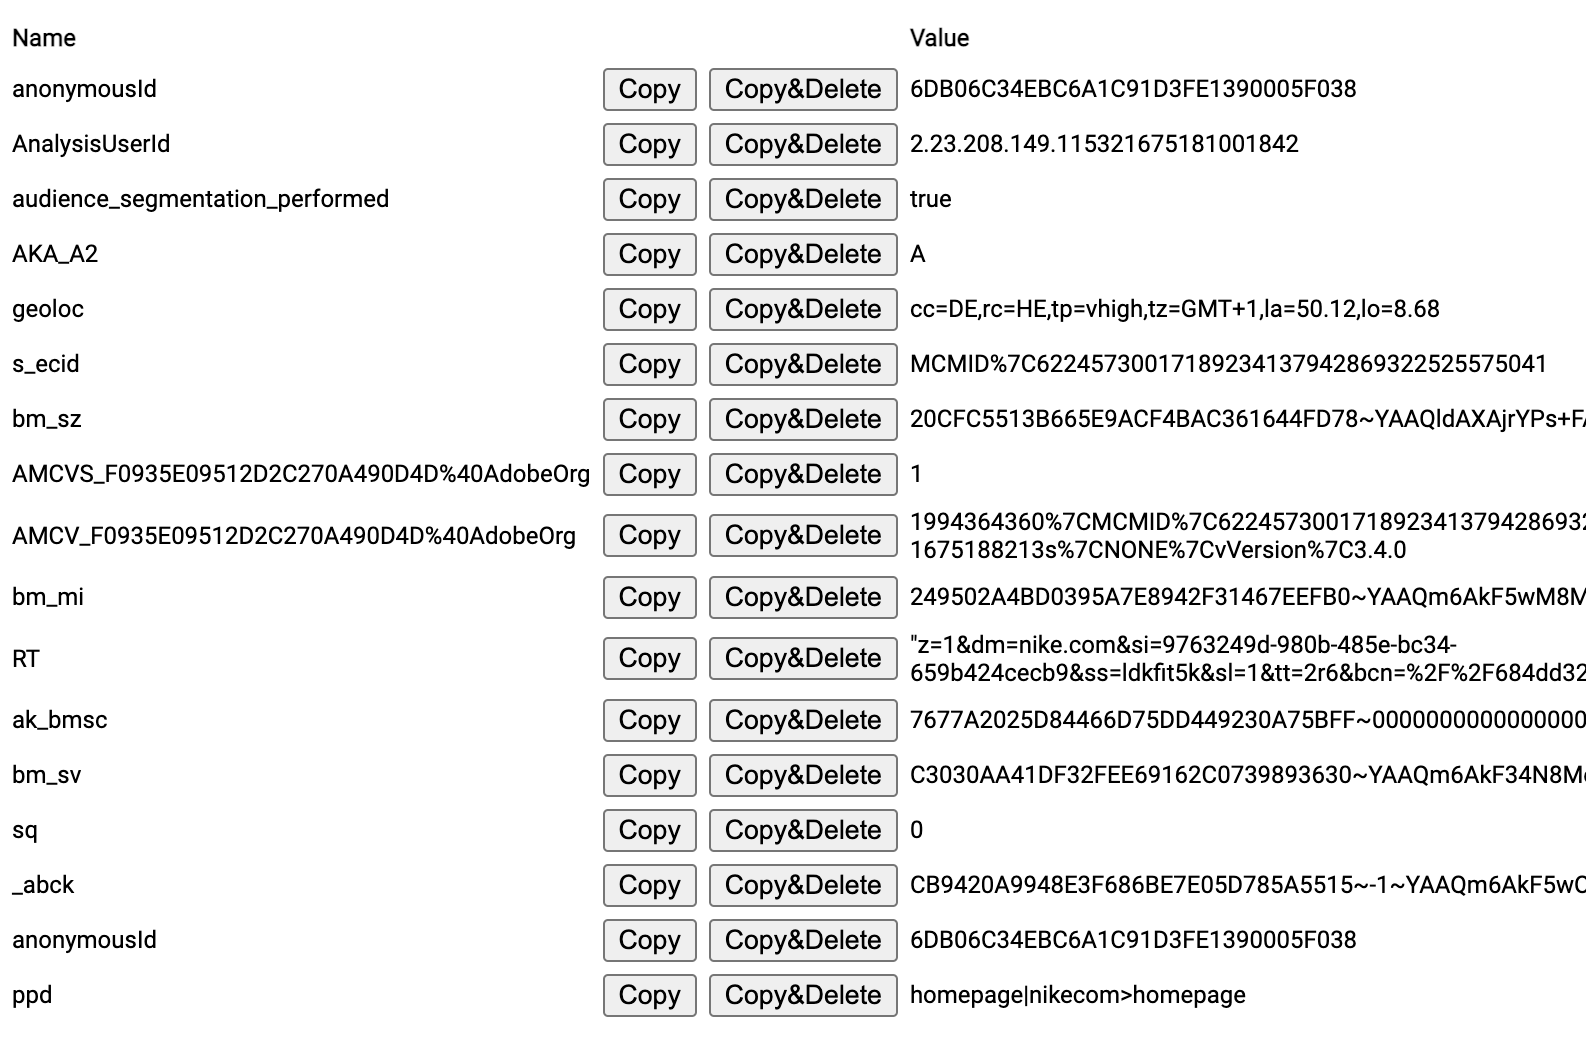
\includegraphics[width=\textwidth]{./gfx/cookiesScreenshot.png}
\centering
\caption{A screenshot of all active cookies being used when visiting \textit{\url{https://www.nike.de}}}
\label{fig:nikeCookies}
\end{figure}

Figure \ref{fig:nikeCookies} shows a screenshot of all active cookies when visiting Nike's German domain. Notice how simply loading their website automatically sets 17 cookies, even before asking for permissions. While some of these may be required for the website to function properly, some may be used to gather information on the visitor. Each key-value pair is encoded, meaning they are not readable for humans. This means that a user is not able to understand what data is being tracked here. Nike may also track similar data on other websites by using third-party cookies.


Gathering users' information in ways that they are not aware of, i.e. through third-parties, begs the question of how long this type of data collection will be possible and if there are any alternative methods to it.


